%!TeX root = main.tex
%!encoding = UTF-8 Unicode

\section{Post-Processing Steps for Extended Emission Analysis}

\subsection{Time-Dependent Noise Filter}

Up to this point, the noise-mitigation steps are generally applicable to arbitrary signals.
Further noise reduction is possible because the EMC-relevant voltage components are concentrated within a limited time interval around the switching event.
Based on this observation, a time-dependent noise filter is introduced that suppresses noise outside the transient, as illustrated for the low-pass signal in Fig.~\ref{fig:TDF}.
This filter is applied to the time-domain signal before the FFT.

\begin{figure}[ht]
	\centering
	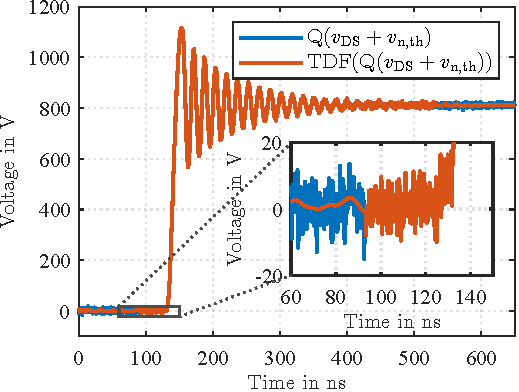
\includegraphics[scale = 1]{figures/3_Methods/TDF/DPT_TD_TDF2.pdf}
	\caption{Time-dependent noise filter to reduce noise outside the switching transient.}\label{fig:TDF}
\end{figure}

First, the transient midpoint \mi{t}{tr} is defined as the time instant at which the drain-source voltage reaches 50\% of its transition between the pre- and post-switching levels.
An asymmetric time window \mi{W}{TDF} is then defined around \mi{t}{tr}. 
Its leading edge extends \mi{T}{TDF}/5 before \mi{t}{tr}, and its trailing edge extends 4\mi{T}{TDF}/5 after \mi{t}{tr}.

\begin{equation}
	\mi{I}{TDF} = \left[\mi{t}{tr}-\frac{\mi{T}{TDF}}{5},\,\mi{t}{tr}+\frac{4\mi{T}{TDF}}{5}\right],
\end{equation}

In this work, the window length \mi{T}{TDF} is set to \SI{500}{ns}, but it should be adjusted to approximately match the observed settling time of the resonant oscillation for the specific device under test.

Afterward, strong filtering is applied only outside the switching transient; within the transient window, the signal remains unfiltered.

\begin{equation}
	\text{TDF}(s) =
	\begin{cases}
		s(t), & t \in \mi{W}{TDF} \\
		\mi{h}{LP,TDF}(t)\ast s(t), & t \notin \mi{W}{TDF}
	\end{cases}
\end{equation}

Here, \mi{h}{LP,TDF} is a second-order Butterworth low-pass filter with a cutoff frequency of \SI{1}{MHz}.
% However, even a stronger filter or a constant setting of the signal to zero outside the switching transient is thinkable.

This filter is applied to the high-pass measurement, while the switching transients are detected in the low-pass measurement.
Thereby, the noise floor is reduced by:

\begin{equation}
	\mi{V}{n,th,TDF} = \frac{\mi{T}{TDF}}{\mi{T}{sw}} \cdot \mi{V}{n,th}
\end{equation}

